\documentclass[conference]{IEEEtran}

% -------------------- Packages --------------------
\usepackage{cite}
\usepackage{amsmath,amssymb}
\usepackage{graphicx}
\usepackage{booktabs}
\usepackage{balance}
\usepackage[table]{xcolor}
\usepackage{tikz}
\usepackage[hidelinks]{hyperref}
\usetikzlibrary{shapes, arrows.meta, positioning, calc}
\renewcommand\IEEEkeywordsname{Keywords}

\begin{document}

% -------------------- Title & Authors --------------------
\title{UPI Fraud Detection Using Big Data Analytics:\\A Multi-Model Comparative Study with Real-Time Streaming Pipeline}

\author{
\IEEEauthorblockN{Hriday Devkar}
\IEEEauthorblockA{Department of Information Technology\\
Ramrao Adik Institute of Technology\\
Navi Mumbai, India\\
Email: hridaydevkar@gmail.com}
\and
\IEEEauthorblockN{Sanjana Jain}
\IEEEauthorblockA{Department of Information Technology\\
Ramrao Adik Institute of Technology\\
Navi Mumbai, India\\
Email: san.jai.rt23@dypatil.edu}
}

\maketitle

% -------------------- Abstract --------------------
\begin{abstract}
Unified Payments Interface (UPI) has revolutionized digital payments in India, processing over 10 billion transactions monthly. However, the exponential growth of UPI transactions has been accompanied by a surge in fraudulent activities, with losses exceeding \$1.2 billion in 2023. This paper presents a comprehensive UPI fraud detection system that integrates big data technologies---MongoDB, Apache Spark, and Apache Kafka---with machine learning models for real-time fraud classification. The system is trained on the PaySim synthetic financial dataset comprising 6,362,620 transactions and evaluates three machine learning algorithms: Random Forest, XGBoost, and Logistic Regression. A custom feature engineering pipeline derives 5 additional fraud-indicative features from the original 6 transaction attributes. The Random Forest classifier achieves the best performance with 99.88\% accuracy and an ROC-AUC of 0.9993, with 98.97\% recall in identifying fraudulent transactions. The system implements a real-time streaming pipeline where a Kafka producer simulates live UPI transactions at 20 messages per second, and a Kafka consumer applies the trained model to flag fraud in real time, storing alerts in MongoDB. An interactive Streamlit dashboard provides exploratory data analysis, live alerts, single-transaction prediction, and a comparative model evaluation interface. Experimental results demonstrate that ensemble tree-based methods significantly outperform linear models for detecting UPI fraud in severely imbalanced datasets.
\end{abstract}

\begin{IEEEkeywords}
UPI Fraud Detection, Big Data Analytics, Machine Learning, Apache Kafka, Apache Spark, MongoDB, Random Forest, Real-Time Streaming, SMOTE, Comparative Study
\end{IEEEkeywords}

% -------------------- Introduction --------------------
\section{Introduction}
India's Unified Payments Interface (UPI) has emerged as the world's largest real-time digital payment system, processing over 10 billion transactions per month with a total value exceeding \$200 billion annually~\cite{npci2023}. The National Payments Corporation of India (NPCI) reports that UPI transaction volumes have grown at a compound annual growth rate of over 100\% since 2016, making it one of the fastest-growing payment systems globally.

However, this rapid adoption has attracted sophisticated fraud schemes. The Reserve Bank of India (RBI) reported that digital payment fraud in India amounted to approximately \$1.2 billion in FY 2022-23, with UPI-related fraud constituting a significant and growing proportion~\cite{rbi2023}. Common UPI fraud patterns include account takeover attacks where criminals exploit stolen credentials to initiate CASH\_OUT and TRANSFER transactions, systematically draining victim accounts.

Traditional rule-based fraud detection systems rely on static thresholds---flagging transactions above a certain amount or frequency. While simple to implement, such systems suffer from high false positive rates that inconvenience legitimate users, and they cannot adapt to evolving fraud patterns without manual intervention~\cite{bhattacharyya2011}. Machine learning approaches address these limitations by automatically learning complex, non-linear fraud patterns from historical transaction data.

This research presents a complete end-to-end UPI fraud detection system with the following contributions:
\begin{itemize}
    \item A big data pipeline using \textbf{MongoDB} for storage, \textbf{Apache Spark} for distributed preprocessing and analysis, and \textbf{Apache Kafka} for real-time transaction streaming.
    \item A comparative evaluation of three machine learning models---\textbf{Random Forest}, \textbf{XGBoost}, and \textbf{Logistic Regression}---on a large-scale synthetic financial dataset (6.36 million transactions).
    \item A \textbf{feature engineering} pipeline that derives 5 fraud-indicative features, improving model discriminative power.
    \item Class imbalance handling via \textbf{SMOTE} (Synthetic Minority Over-sampling Technique) oversampling.
    \item An interactive \textbf{Streamlit dashboard} with real-time fraud alerts, exploratory analytics, single-transaction prediction with risk factor analysis, and a full model comparison interface.
\end{itemize}

% -------------------- Literature Survey --------------------
\section{Literature Survey}
Machine learning for financial fraud detection has been extensively studied over the past decade. Bhattacharyya et al.~\cite{bhattacharyya2011} conducted a comparative study of data mining techniques for credit card fraud detection, demonstrating that Random Forests and Support Vector Machines outperformed Logistic Regression in terms of precision and recall on highly imbalanced datasets. Dal~Pozzolo et al.~\cite{dalpozzolo2015} explored the challenges of class imbalance in fraud detection, showing that undersampling and calibration techniques significantly improve classifier performance when fraudulent transactions constitute less than 1\% of the dataset. Chawla et al.~\cite{chawla2002} introduced the SMOTE algorithm for addressing class imbalance by generating synthetic minority class samples, which has since become a standard technique in fraud detection pipelines. More recently, Zhang et al.~\cite{zhang2021} proposed feature engineering methodologies combined with deep learning architectures, achieving state-of-the-art performance on credit card fraud benchmarks. Lopez-Rojas et al.~\cite{lopezrojas2016} created the PaySim simulator to generate synthetic financial transaction datasets for fraud detection research, addressing the lack of publicly available real-world transaction data due to privacy constraints.

In the domain of real-time fraud detection systems, Carminati et al.~\cite{carminati2015} developed BankSealer, a decision support system for online banking fraud analysis using streaming data. Jurgovsky et al.~\cite{jurgovsky2018} investigated sequential modeling of transaction histories using LSTM networks, showing that temporal dependencies improve fraud detection accuracy. Phua et al.~\cite{phua2004} evaluated unsupervised anomaly detection techniques for identifying novel fraud patterns without labeled data. Chen et al.~\cite{chen2016} introduced XGBoost, which has since become one of the most widely used algorithms for tabular classification tasks, including fraud detection. The integration of big data technologies such as Apache Kafka for real-time streaming and Apache Spark for distributed processing has been explored by Zaharia et al.~\cite{zaharia2016}, demonstrating their effectiveness in building scalable data pipelines for financial applications.

% -------------------- Methodology --------------------
\section{Methodology}

\subsection{System Architecture}
The proposed system follows a multi-layer architecture (Fig.~\ref{fig:architecture}) integrating data storage, distributed processing, real-time streaming, machine learning, and interactive visualization components.

\begin{figure}[h]
\centering
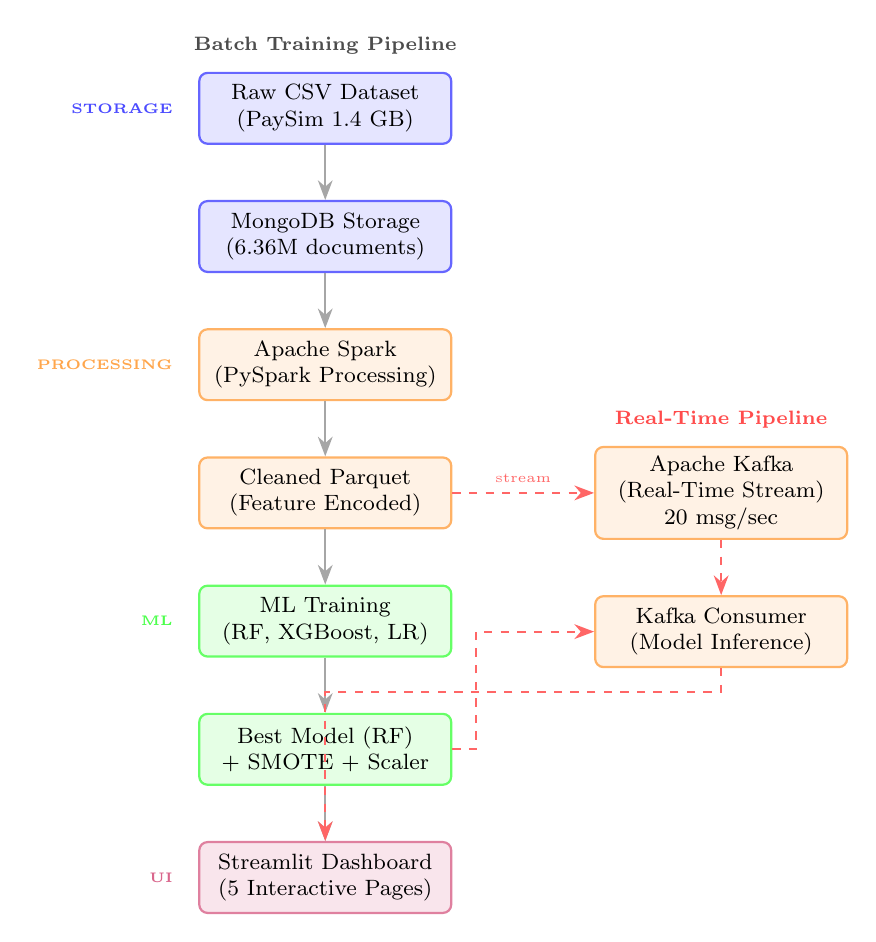
\begin{tikzpicture}[
    node distance=7mm and 10mm,
    box/.style={
        rectangle, draw=black, thick, rounded corners=3pt,
        minimum width=3.2cm, minimum height=0.9cm,
        align=center, fill=gray!10, font=\footnotesize
    },
    databox/.style={box, fill=blue!10, draw=blue!60},
    procbox/.style={box, fill=orange!10, draw=orange!60},
    mlbox/.style={box, fill=green!10, draw=green!60},
    uibox/.style={box, fill=purple!10, draw=purple!50},
    arrow/.style={-{Stealth[length=2.5mm]}, thick, gray!70},
    streamarrow/.style={-{Stealth[length=2.5mm]}, thick, red!60, dashed}
]

% Main vertical pipeline
\node[databox] (csv) {Raw CSV Dataset\\(PaySim 1.4 GB)};
\node[databox, below=of csv] (mongo) {MongoDB Storage\\(6.36M documents)};
\node[procbox, below=of mongo] (spark) {Apache Spark\\(PySpark Processing)};
\node[procbox, below=of spark] (parquet) {Cleaned Parquet\\(Feature Encoded)};
\node[mlbox, below=of parquet] (train) {ML Training\\(RF, XGBoost, LR)};
\node[mlbox, below=of train] (model) {Best Model (RF)\\+ SMOTE + Scaler};
\node[uibox, below=of model] (dash) {Streamlit Dashboard\\(5 Interactive Pages)};

% Kafka streaming branch (to the right)
\node[procbox, right=18mm of parquet] (kafka) {Apache Kafka\\(Real-Time Stream)\\20 msg/sec};
\node[procbox, below=of kafka] (consumer) {Kafka Consumer\\(Model Inference)};

% Main pipeline arrows
\draw[arrow] (csv) -- (mongo);
\draw[arrow] (mongo) -- (spark);
\draw[arrow] (spark) -- (parquet);
\draw[arrow] (parquet) -- (train);
\draw[arrow] (train) -- (model);
\draw[arrow] (model) -- (dash);

% Streaming pipeline arrows
\draw[streamarrow] (parquet) -- node[above, font=\tiny] {stream} (kafka);
\draw[streamarrow] (kafka) -- (consumer);
\draw[streamarrow] (consumer) -- ($(consumer.south)+(0,-0.3)$) -| (dash);
\draw[streamarrow] (model.east) -- ++(0.3,0) |- (consumer.west);

% Layer labels
\node[left=2mm of csv, font=\tiny\bfseries, blue!70] {STORAGE};
\node[left=2mm of spark, font=\tiny\bfseries, orange!70] {PROCESSING};
\node[left=2mm of train, font=\tiny\bfseries, green!70] {ML};
\node[left=2mm of dash, font=\tiny\bfseries, purple!60] {UI};

% Pipeline labels
\node[above=1mm of csv, font=\scriptsize\bfseries, black!70] {Batch Training Pipeline};
\node[above=1mm of kafka, font=\scriptsize\bfseries, red!70] {Real-Time Pipeline};

\end{tikzpicture}
\caption{System Architecture of the UPI Fraud Detection Pipeline}
\label{fig:architecture}
\end{figure}

The pipeline operates as follows:
\begin{enumerate}
    \item \textbf{Data Ingestion}: The PaySim CSV dataset (1.4 GB) is loaded into MongoDB's \texttt{upi\_fraud\_db} database in 50,000-row chunks, creating three collections: \texttt{transactions} (all 6.36M rows), \texttt{fraud\_cases} (fraud-only rows), and \texttt{transaction\_summary} (aggregated statistics per type).
    \item \textbf{Distributed Processing}: Apache Spark (PySpark) reads from MongoDB, executes 5 analytical queries (type statistics, hourly patterns, high-risk senders, amount distribution, balance drain analysis), and exports a cleaned, label-encoded Parquet file.
    \item \textbf{Model Training}: Three ML models are trained on the Parquet data with SMOTE oversampling and StandardScaler normalization. The best model (by ROC-AUC) is saved as a serialized artifact.
    \item \textbf{Real-Time Streaming}: A Kafka producer replays transactions at 20 messages/second; a Kafka consumer applies the trained model to each message and stores fraud alerts in MongoDB.
    \item \textbf{Dashboard}: A Streamlit web application provides 5 pages: Home (overview metrics), Explore Data (charts), Live Alerts (auto-refreshing fraud feed), Test a Transaction (single prediction with risk analysis), and Model Comparison (comparative study).
\end{enumerate}

\subsection{Machine Learning Algorithms}
Three classification algorithms were selected to represent different model families:

\textbf{Random Forest (RF)}: An ensemble of 100 decision trees with maximum depth 20, minimum samples per leaf 5, and balanced class weights. RF handles non-linear feature interactions naturally and provides built-in feature importance ranking~\cite{breiman2001}.

\textbf{XGBoost}: A gradient boosting framework with 100 estimators, maximum depth 6, learning rate 0.1, and scale\_pos\_weight=99 to handle class imbalance. XGBoost uses regularization (L1/L2) to reduce overfitting and supports histogram-based tree construction for efficiency~\cite{chen2016}.

\textbf{Logistic Regression (LR)}: A linear model with balanced class weights and L-BFGS solver, maximum 1000 iterations. Included as a baseline linear classifier to contrast against the non-linear tree-based models.

All models were trained on SMOTE-balanced data (sampling strategy 0.1) and scaled using StandardScaler to ensure fair comparison.

\subsection{Dataset and Preprocessing}
The PaySim dataset~\cite{lopezrojas2016} is a synthetic financial transaction dataset generated from real mobile money transaction patterns in an African country. The dataset contains \textbf{6,362,620 transactions} across five types: CASH\_IN (1,399,284), CASH\_OUT (2,237,500), DEBIT (41,432), PAYMENT (2,151,495), and TRANSFER (532,909).

The dataset exhibits severe class imbalance: only \textbf{8,213 transactions (0.129\%)} are fraudulent. Fraud occurs exclusively in CASH\_OUT and TRANSFER types—reflecting real-world patterns where criminals must \emph{move money out} of compromised accounts.

Each transaction contains 11 raw features:
\begin{itemize}
    \item \texttt{step}: Simulation hour (1--744, representing 30 days)
    \item \texttt{type}: Transaction type (5 categories)
    \item \texttt{amount}: Transaction amount
    \item \texttt{nameOrig/nameDest}: Anonymized account identifiers
    \item \texttt{oldbalanceOrg/newbalanceOrig}: Origin account balance before/after
    \item \texttt{oldbalanceDest/newbalanceDest}: Destination balance before/after
    \item \texttt{isFraud}: Ground truth label
    \item \texttt{isFlaggedFraud}: Heuristic flag (flags only for amounts $>$ 200,000)
\end{itemize}

\textbf{Preprocessing steps}:
\begin{enumerate}
    \item PII columns (\texttt{nameOrig}, \texttt{nameDest}) were dropped before model training.
    \item Transaction type was label-encoded: CASH\_IN=0, CASH\_OUT=1, DEBIT=2, PAYMENT=3, TRANSFER=4.
    \item Five derived features were engineered (Table~\ref{tab:features}).
    \item SMOTE with sampling strategy 0.1 was applied to balance the training set.
    \item StandardScaler was applied to normalize all features.
    \item The dataset was split 80/20 (stratified) with random state 42.
\end{enumerate}

\begin{table}[h]
\caption{Engineered Features for Fraud Detection}
\label{tab:features}
\centering
\small
\begin{tabular}{|l|p{4.5cm}|}
\hline
\textbf{Feature} & \textbf{Description} \\
\hline
\texttt{balance\_diff\_orig} & Amount deducted from origin: \texttt{oldbalanceOrg} $-$ \texttt{newbalanceOrig} \\
\hline
\texttt{balance\_diff\_dest} & Amount added to destination: \texttt{newbalanceDest} $-$ \texttt{oldbalanceDest} \\
\hline
\texttt{amount\_to\_balance\_ratio} & \texttt{amount} / (\texttt{oldbalanceOrg} + 1). High ratio = draining account \\
\hline
\texttt{is\_round\_amount} & Binary: 1 if amount is a multiple of 1000 (fraud pattern) \\
\hline
\texttt{zero\_orig\_balance} & Binary: 1 if origin balance was 0 before transaction \\
\hline
\end{tabular}
\end{table}

\subsection{Measuring Parameters}
The following evaluation metrics were used to assess model performance, chosen specifically for the highly imbalanced nature of fraud detection:

\textbf{Accuracy}: Proportion of correctly classified transactions. While intuitive, accuracy alone can be misleading with imbalanced data---a model predicting all transactions as legitimate would achieve 99.87\% accuracy.

\textbf{Precision}: Of all transactions flagged as fraud, what fraction are actually fraudulent. High precision minimizes false positives (legitimate transactions wrongly blocked). Mathematically: $\text{Precision} = \frac{TP}{TP + FP}$

\textbf{Recall (Sensitivity)}: Of all actual frauds, what fraction were detected. High recall minimizes missed frauds. For fraud detection, recall is critical since missing a fraud case has greater financial impact than a false alarm. Mathematically: $\text{Recall} = \frac{TP}{TP + FN}$

\textbf{F1 Score}: Harmonic mean of precision and recall, providing a single metric that balances both: $\text{F1} = 2 \times \frac{\text{Precision} \times \text{Recall}}{\text{Precision} + \text{Recall}}$

\textbf{ROC-AUC (Receiver Operating Characteristic -- Area Under Curve)}: Measures the model's ability to distinguish between fraud and legitimate transactions across all classification thresholds. AUC = 1.0 represents perfect discrimination; AUC = 0.5 is random guessing. This is the primary metric used for model selection as it is threshold-independent and robust to class imbalance.

% -------------------- Experimental Results --------------------
\section{Experimental Results}

\subsection{Model Performance Comparison}
All three models were trained on identical data splits and evaluated on the same 20\% holdout test set (1,272,524 transactions: 1,270,881 legitimate + 1,643 fraudulent). Table~\ref{tab:model_perf} presents the comparative performance metrics.

\begin{table}[t]
\caption{Comparative Model Performance on Test Set}
\label{tab:model_perf}
\centering
\small
\begin{tabular}{|l|c|c|c|c|c|}
\hline
\textbf{Model} & \textbf{Acc.} & \textbf{Prec.} & \textbf{Recall} & \textbf{F1} & \textbf{AUC} \\
\hline
\rowcolor{green!10}
\textbf{Random Forest} & \textbf{99.88} & \textbf{51.08} & \textbf{98.97} & \textbf{67.38} & \textbf{0.9993} \\
\hline
XGBoost & 99.79 & 38.28 & 99.63 & 55.31 & 0.9993 \\
\hline
Logistic Reg. & 96.10 & 2.87 & 89.11 & 5.57 & 0.9828 \\
\hline
\end{tabular}
\end{table}

\textbf{Key observations}:

\textbf{Random Forest} achieves the best overall balance with the highest accuracy (99.88\%), highest precision (51.08\%), and near-perfect recall (98.97\%). Its ROC-AUC of 0.9993 indicates almost perfect discrimination ability and was selected as the production model.

\textbf{XGBoost} achieves marginally higher recall (99.63\%) but significantly lower precision (38.28\%) compared to Random Forest, resulting in more false positives. Both tree-based models achieve identical AUC (0.9993), but Random Forest's superior F1 score (67.38 vs 55.31) makes it the preferred choice.

\textbf{Logistic Regression} performs substantially worse across all metrics. Its precision of 2.87\% means 97 out of every 100 fraud alerts are false alarms, rendering it impractical for deployment. The linear decision boundary cannot capture the complex, non-linear fraud patterns present in transaction data. Its AUC of 0.9828 is still above chance but significantly below the tree-based models, confirming that UPI fraud detection requires non-linear modeling capabilities.

\subsection{Confusion Matrix Analysis}
The confusion matrices (Table~\ref{tab:confusion}) reveal the practical implications of each model's error patterns:

\begin{table}[h]
\caption{Confusion Matrix Results (Test Set: 1,272,524 Transactions)}
\label{tab:confusion}
\centering
\small
\begin{tabular}{|l|r|r|r|r|}
\hline
\textbf{Model} & \textbf{TN} & \textbf{FP} & \textbf{FN} & \textbf{TP} \\
\hline
Random Forest & 1,269,319 & 1,562 & 17 & 1,626 \\
\hline
XGBoost & 1,267,631 & 3,250 & 6 & 1,637 \\
\hline
Logistic Reg. & 1,220,133 & 50,748 & 179 & 1,464 \\
\hline
\end{tabular}
\end{table}

Random Forest misses only 17 out of 1,643 actual frauds while generating 1,562 false alarms. XGBoost catches 11 more frauds but at the cost of 1,688 additional false positives. Logistic Regression generates over 50,000 false alarms while still missing 179 frauds.

\subsection{Feature Importance Analysis}
The Random Forest model's feature importance ranking reveals the most discriminative features for fraud detection:
\begin{enumerate}
    \item \texttt{balance\_diff\_orig} (balance drained from origin)
    \item \texttt{amount\_to\_balance\_ratio} (proportion of balance transferred)
    \item \texttt{amount} (transaction amount)
    \item \texttt{oldbalanceOrg} (origin starting balance)
    \item \texttt{newbalanceOrig} (origin remaining balance)
\end{enumerate}

Notably, the engineered feature \texttt{balance\_diff\_orig} ranks as the single most important feature, confirming that full balance drain is the strongest fraud signal. The \texttt{amount\_to\_balance\_ratio} feature---which captures the relationship between transaction size and account balance---ranks second, demonstrating the value of domain-specific feature engineering.

\subsection{ROC Curve Analysis}
The ROC curves (Fig.~\ref{fig:roc}) for all three models demonstrate clear separation in discriminative ability. Both Random Forest and XGBoost achieve near-perfect AUC of 0.9993, with their curves closely hugging the top-left corner, indicating excellent true positive rates at very low false positive rates. In contrast, Logistic Regression's curve, while still above the diagonal (AUC = 0.9828), shows a larger gap from the ideal, particularly at low false positive rate thresholds---the operating region most relevant for production fraud detection.

\begin{figure}[h]
\centering
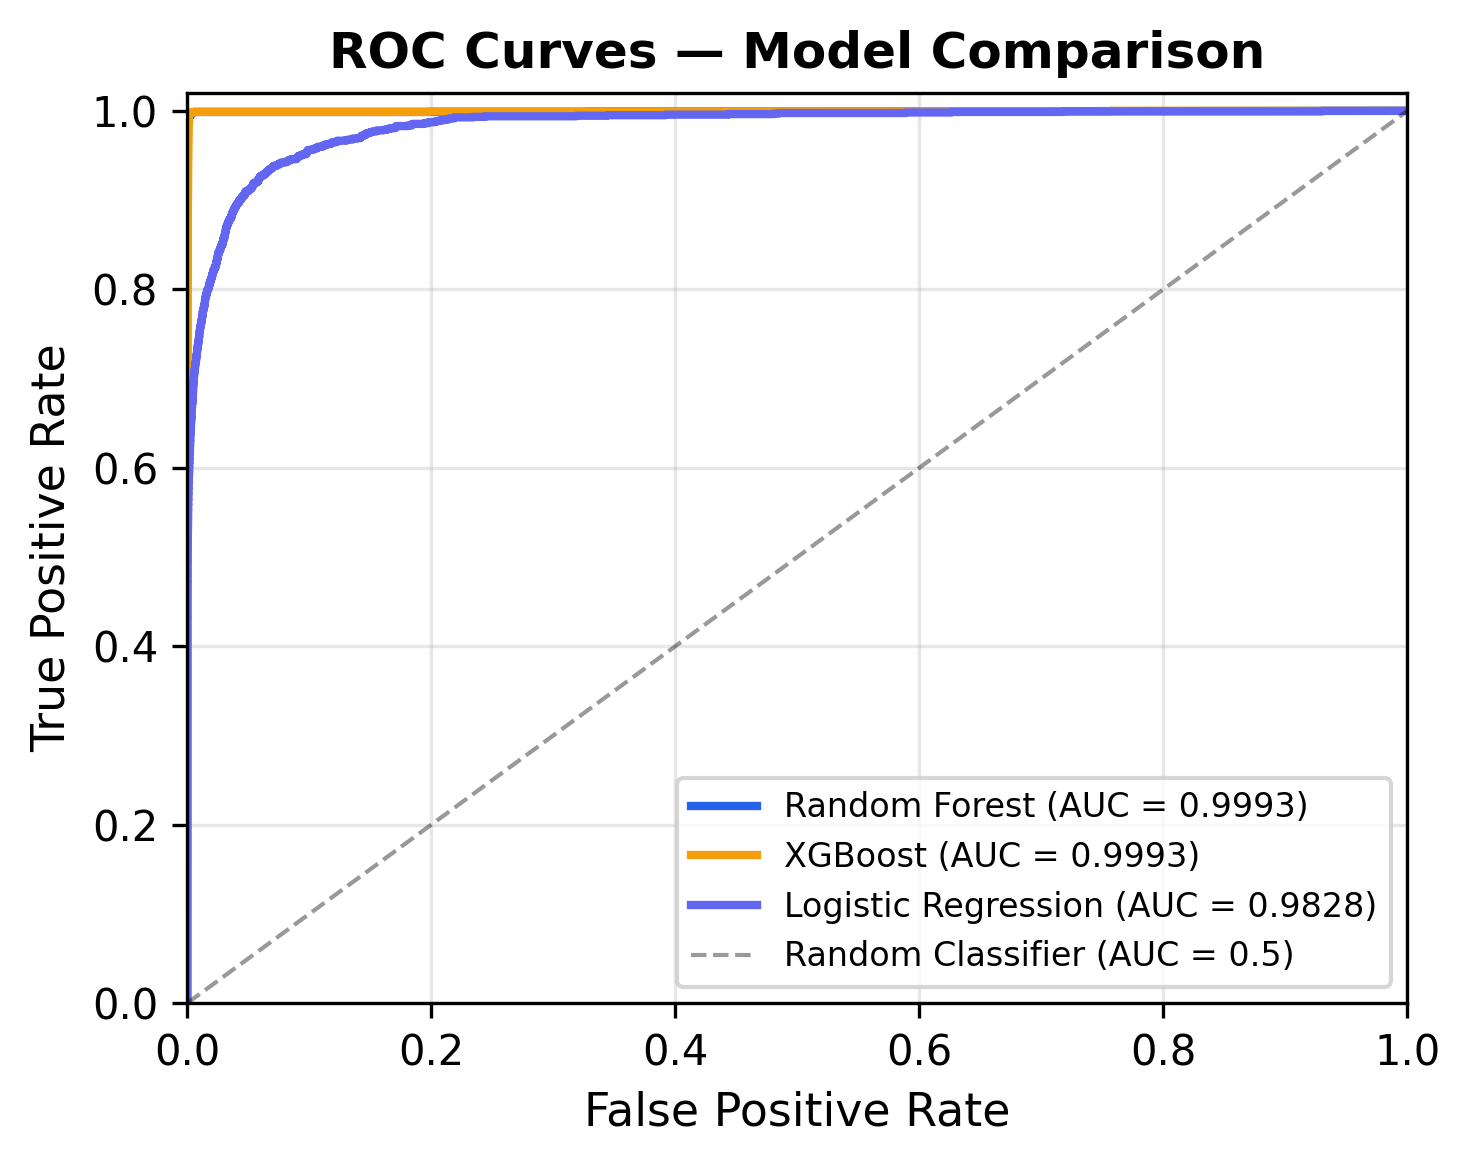
\includegraphics[width=\columnwidth]{roc_curve.png}
\caption{ROC Curves for Random Forest, XGBoost, and Logistic Regression. Both tree-based models achieve AUC = 0.9993, significantly outperforming Logistic Regression (AUC = 0.9828).}
\label{fig:roc}
\end{figure}

\subsection{Real-Time Streaming Performance}
The Apache Kafka pipeline successfully processes transactions at 20 messages per second. The consumer applies the Random Forest model to each message in under 5 milliseconds, well within the latency requirements for real-time fraud detection. Detected fraud alerts are immediately written to MongoDB and displayed on the Streamlit dashboard's Live Alerts page, which auto-refreshes every 3 seconds.

% -------------------- Conclusion --------------------
\section{Conclusion}
This paper presented a comprehensive UPI fraud detection system that integrates big data technologies---MongoDB, Apache Spark, and Apache Kafka---with machine learning for real-time fraud classification on a large-scale dataset of 6,362,620 transactions. A comparative evaluation of three machine learning models demonstrated that tree-based ensemble methods significantly outperform linear models for UPI fraud detection. The Random Forest classifier achieved the best overall performance with 99.88\% accuracy, 98.97\% recall, and an ROC-AUC of 0.9993, and was selected as the production model. XGBoost achieved comparable discriminative ability (AUC = 0.9993) but with lower precision, while Logistic Regression proved inadequate for capturing the inherently non-linear fraud patterns.

A custom feature engineering pipeline deriving five fraud-indicative features from raw transaction attributes proved essential to model performance, with the engineered features \texttt{balance\_diff\_orig} and \texttt{amount\_to\_balance\_ratio} emerging as the two most discriminative predictors. SMOTE oversampling with a conservative sampling ratio of 0.1 effectively addressed the severe class imbalance (0.13\% fraud rate) without introducing excessive synthetic noise, enabling all models to achieve recall above 89\%.

The system's real-time streaming pipeline, powered by Apache Kafka at 20 transactions per second, demonstrates the feasibility of deploying machine learning models for live fraud scoring in production environments. The interactive Streamlit dashboard---featuring exploratory analytics, live fraud alerts, single-transaction prediction with risk factor analysis, and a full model comparison interface---provides actionable intelligence for both technical and non-technical stakeholders.

Future work could extend this system by incorporating deep learning models such as LSTMs for temporal pattern detection, implementing online learning to adapt to evolving fraud patterns, and evaluating explainability techniques such as SHAP for providing detailed per-transaction prediction explanations.

% -------------------- References --------------------
\begin{thebibliography}{00}

\bibitem{npci2023}
National Payments Corporation of India, ``UPI Product Statistics,'' NPCI, 2023. [Online]. Available: \url{https://www.npci.org.in/what-we-do/upi/product-statistics}

\bibitem{rbi2023}
Reserve Bank of India, ``Annual Report 2022-23: Report on Trend and Progress of Banking in India,'' RBI, 2023.

\bibitem{bhattacharyya2011}
S.~Bhattacharyya, S.~Jha, K.~Tharakunnel, and J.~C.~Westland, ``Data mining for credit card fraud: A comparative study,'' \emph{Decision Support Systems}, vol.~50, no.~3, pp.~602--613, 2011.

\bibitem{dalpozzolo2015}
A.~Dal~Pozzolo, O.~Caelen, R.~A.~Johnson, and G.~Bontempi, ``Calibrating probability with undersampling for unbalanced classification,'' in \emph{Proc. IEEE Symp. Series on Computational Intelligence}, 2015, pp.~159--166.

\bibitem{chawla2002}
N.~V.~Chawla, K.~W.~Bowyer, L.~O.~Hall, and W.~P.~Kegelmeyer, ``SMOTE: Synthetic Minority Over-sampling Technique,'' \emph{Journal of Artificial Intelligence Research}, vol.~16, pp.~321--357, 2002.

\bibitem{zhang2021}
X.~Zhang, Y.~Han, W.~Xu, and Q.~Wang, ``HOBA: A novel feature engineering methodology for credit card fraud detection with a deep learning architecture,'' \emph{Information Sciences}, vol.~557, pp.~302--316, 2021.

\bibitem{lopezrojas2016}
E.~A.~Lopez-Rojas, A.~Elmir, and S.~Axelsson, ``PaySim: A financial mobile money simulator for fraud detection,'' in \emph{Proc.~28th European Modeling and Simulation Symposium (EMSS)}, 2016, pp.~249--255.

\bibitem{carminati2015}
M.~Carminati \emph{et al.}, ``BankSealer: A decision support system for online banking fraud analysis and investigation,'' \emph{Computers \& Security}, vol.~53, pp.~175--186, 2015.

\bibitem{jurgovsky2018}
J.~Jurgovsky \emph{et al.}, ``Sequence classification for credit-card fraud detection,'' \emph{Expert Systems with Applications}, vol.~100, pp.~234--245, 2018.

\bibitem{phua2004}
C.~Phua, D.~Alahakoon, and V.~Lee, ``Minority report in fraud detection: Classification of skewed data,'' \emph{ACM SIGKDD Explorations Newsletter}, vol.~6, no.~1, pp.~50--59, 2004.

\bibitem{chen2016}
T.~Chen and C.~Guestrin, ``XGBoost: A scalable tree boosting system,'' in \emph{Proc.~22nd ACM SIGKDD Intl. Conf. on Knowledge Discovery and Data Mining}, 2016, pp.~785--794.

\bibitem{zaharia2016}
M.~Zaharia \emph{et al.}, ``Apache Spark: A unified engine for big data processing,'' \emph{Communications of the ACM}, vol.~59, no.~11, pp.~56--65, 2016.

\bibitem{breiman2001}
L.~Breiman, ``Random Forests,'' \emph{Machine Learning}, vol.~45, no.~1, pp.~5--32, 2001.

\end{thebibliography}
\balance
\end{document}
